\section*{Networks}

    Now, we have fully developed the individual \textbf{neuron}. 
    
    We can even do \textbf{gradient descent} on it: just like when we were doing LLCs, we can use the \textbf{chain rule}. 
        \note{We'll get into this more, later in the chapter.}
        
    So, we return to the idea from the beginning of this chapter: combining multiple neurons into a \textbf{network}. 
    
    \subsection*{Abstraction}
        For this next section, we'll \textbf{simplify} the above diagram to this:
        
        \begin{figure}[H]
            \centering
            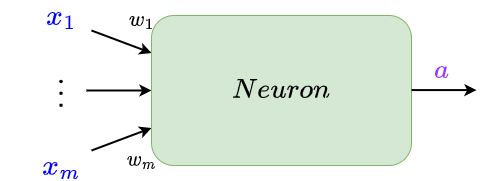
\includegraphics[width=60mm,scale=0.4]{images/nn_images/neuron_abstraction.png}
        \end{figure}
        
        In fact, for more \textbf{simplicity}, we'll draw \textbf{one} arrow to represent the whole vector $x$. However, nothing about the \textbf{actual} math has changed.
        
        \begin{figure}[H]
            \centering
            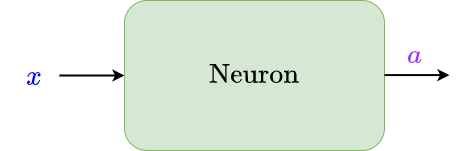
\includegraphics[width=50mm,scale=0.4]{images/nn_images/neuron_abstraction_x.png}
        \end{figure}
        
        This is also called \textbf{abstraction} - we need it a lot in this chapter.\\
        
        \begin{definition}
            \vocab{Abstraction} is a way to view your system more \gren{broadly}: removing excess details, to make it \gren{easier} to work with.
            
            Abstraction takes a \purp{complicated} system, and focuses on only the \purp{important} details. Everything else is \gren{excluded} from the model.
            
            Often, this \purp{simplified} view boils a system down to its the \gren{inputs} and \gren{outputs}: the "interface".
        \end{definition}
        
        \miniex Rather than thinking about all of the \textbf{mechanics} of how a car works, you might \textbf{abstract} it down to the pedals, the steering wheel, and how that causes the car to move.
    
    \subsection*{Some limitations: acyclic networks}
    
        We won't allow for just \textbf{any} kind of network: we can create ones that might be unhelpful, or just very \textbf{difficult} to \textbf{analyze}. 
        
        For now, we can get interesting and \textbf{useful} behavior while keeping it \textbf{systematic}. We'll define this "system" later.
    
        We'll assume our networks are \textbf{acyclic}: they do not create closed \textbf{loops}, where something can affects it own input.
        
        \begin{figure}[H]
            \centering
            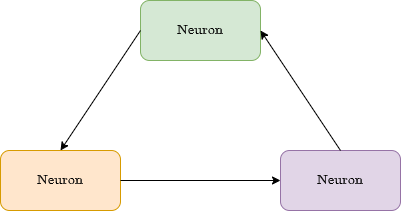
\includegraphics[width=100mm,scale=0.4]{images/nn_images/cyclic_network.png}
            \caption*{This is a cyclic network: this is messy and we won't worry about this for now.}
        \end{figure}
        
        This means information only \textbf{flows} in one direction, "forward": it never flows "backwards".\\
        
        \begin{concept}
            For simple \vocab{neural networks}, we assume that they are \purp{acyclic}: there are no \gren{cycles}, or loops.
            
            This means that \purp{no neuron} has an output that affects its \gren{input}, directly or indirectly.
            
            We call these \vocab{feed-forward} networks.
        \end{concept}
        
        We'll show how to build up the rest of what we need.
    
    \subsection*{How to build networks}
        
        Suppose we have two neuron in \textbf{series}, our \textbf{simplest} arrangement:
        
        \begin{figure}[H]
            \centering
            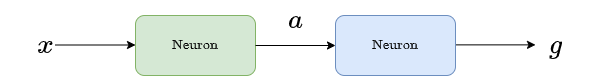
\includegraphics[width=100mm,scale=0.4]{images/nn_images/series_a.png}
        \end{figure}
        
        Our first neuron takes in a whole \textbf{vector} of values, $x = [x_1, x_2, ..., x_m]^T$. But, it only \textbf{outputs} a single value, $a$.
            \note{Remember that while we only see one arrow from $x$, each data point $x_i$ is included.}
        
        That means the second neuron only receives \textbf{one} value, but it's capable of handling a full \textbf{vector}. We can add more values!
        
        Let's add \textbf{another} neuron.
        
        \begin{figure}[H]
            \centering
            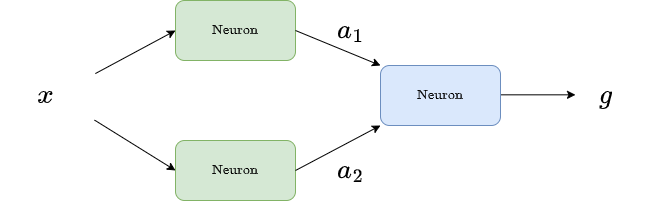
\includegraphics[width=100mm,scale=0.4]{images/nn_images/two_neurons_a.png}
        \end{figure}
        
        Our rightmost neuron now has \textbf{2 inputs}, which can be stored in a vector,
        
        \begin{equation}
            A = 
            \begin{bmatrix}
              a_1 \\ a_2
            \end{bmatrix}
        \end{equation}
        
        We could increase the \textbf{length} of this vector by adding more \textbf{neurons}.
        
        \begin{figure}[H]
            \centering
            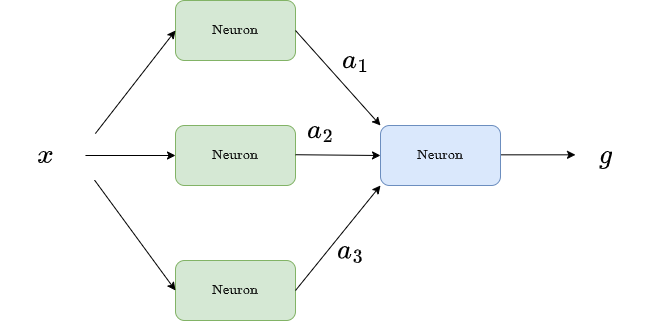
\includegraphics[width=100mm,scale=0.4]{images/nn_images/three_parallel.png}
        \end{figure}
        
        \begin{equation}
            A = \begin{bmatrix}
              a_1 \\ a_2 \\ a_3
            \end{bmatrix}
        \end{equation}
        
        For our \textbf{rightmost} neuron, this is effectively the \textbf{same} as $x$: an \textbf{input vector}. 
        
    \subsection*{Layers}
        
        This gives us an idea for how to \textbf{build} our network: using multiple neurons in \textbf{parallel}, we can output a new vector $A$! 
        
        This is useful, because it means we can \textbf{simplify}: from the rightmost neuron's perspective, it just sees that \textbf{vector} as an input.
        
        \begin{figure}[H]
            \centering
            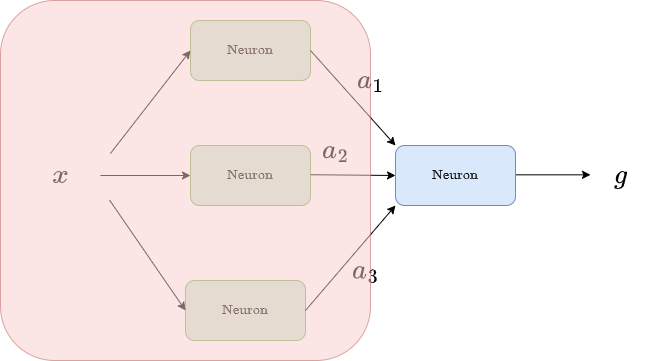
\includegraphics[width=80mm,scale=0.4]{images/nn_images/abstracting_A.png}
            \caption*{We can take this entire layer...}
        \end{figure}
        
        \begin{figure}[H]
            \centering
            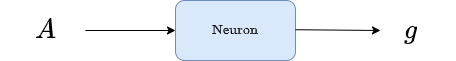
\includegraphics[width=80mm,scale=0.4]{images/nn_images/second_layer.png}
            \caption*{And just reduce it down to the vector $A$.}
        \end{figure}

        Because it's so useful, we'll give this set of neurons a name: a \textbf{layer}.\\
        
        \begin{definition}
            A \vocab{layer} is a set of \gren{neurons} that are in "parallel":
            \begin{itemize}
                \item They all have \gren{inputs} from the same \purp{previous layer}
                    \begin{itemize}
                        \item This \purp{previous layer} could also be the \gren{original input} $x$.
                    \end{itemize}
                
                \item They all have \gren{outputs} to the same \purp{next layer}
                    \begin{itemize}
                        \item This \purp{next layer} could also be the \gren{final output} of the neural network.
                    \end{itemize}
                
                \item And none of these neurons are directly \purp{connected} to each other.
            \end{itemize}
        \end{definition}
        
        This \textbf{layering} structure allows us to simplify our \textbf{analysis}: anything that comes after the layer only has to work with a \textbf{single vector}.
        
        A layer in general might looks like this:
        
        \begin{figure}[H]
            \centering
            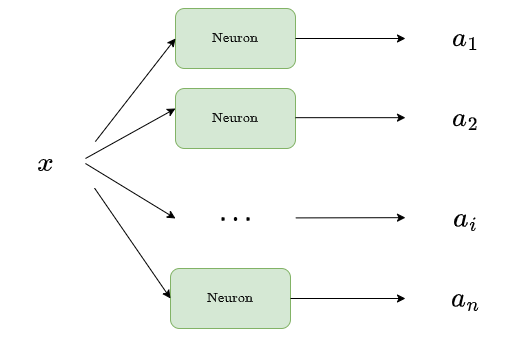
\includegraphics[width=80mm,scale=0.4]{images/nn_images/general_layer.png}
            \caption*{A general layer in a neural network.}
        \end{figure}
        
    \subsection*{The Basic Structure of a Neural Network}
        
        We could pick many structures for neural networks, but for simplicity, this will define our \textbf{template} for this chapter.\\
        
        \begin{definition}
            We structure our \vocab{neural networks} as a series of \purp{layers}, where each layer is the \gren{input} to the next layer.
            
            This means that \purp{layers} are a basic unit of a neural network, one level above a \gren{neuron}.
        \end{definition}
        
        In short, we have:
        
        \begin{itemize}
            \item A \vocab{neuron}, made of a linear and an activation component
            
            \item A \vocab{layer}, made of many neurons in parallel
            
            \item A \vocab{neural} network, made of many layers in series
        \end{itemize}
        
        Our goal is some kind of structure that looks something like this:
        
        \begin{figure}[H]
            \centering
            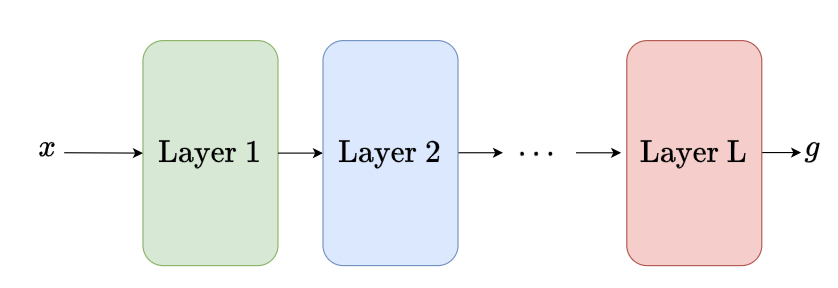
\includegraphics[width=100mm,scale=0.4]{images/nn_images/layers.png}
            \caption*{A neural network.}
        \end{figure}
        
        We now have a high-level view of our entire neural network, so now we dig into the details of a single layer.
        
        